%Notes by Harsh Mistry 
%CS 370
%Based on Template From  https://www.cs.cmu.edu/~ggordon/10725-F12/template.tex

\documentclass[twoside]{article}
\setlength{\oddsidemargin}{0.25 in}
\setlength{\evensidemargin}{-0.25 in}
\setlength{\topmargin}{-0.6 in}
\setlength{\textwidth}{6.5 in}
\setlength{\textheight}{8.5 in}
\setlength{\headsep}{0.75 in}
\setlength{\parindent}{0 in}
\setlength{\parskip}{0.1 in}
\usepackage{amsfonts,graphicx, amssymb}
\usepackage[fleqn]{amsmath}
\usepackage{fixltx2e}
\usepackage{color}
\usepackage{tcolorbox}
\usepackage{lipsum}
\usepackage{listings}
\usepackage{scrextend}
\tcbuselibrary{skins,breakable}
\usetikzlibrary{shadings,shadows}
\newcounter{lecnum}
\renewcommand{\thepage}{\thelecnum-\arabic{page}}
\renewcommand{\thesection}{\thelecnum.\arabic{section}}
\renewcommand{\theequation}{\thelecnum.\arabic{equation}}
\renewcommand{\thefigure}{\thelecnum.\arabic{figure}}
\renewcommand{\thetable}{\thelecnum.\arabic{table}}
\newcommand{\lecture}[4]{
   \pagestyle{myheadings}
   \thispagestyle{plain}
   \newpage
   \setcounter{lecnum}{#1}
   \setcounter{page}{1}
   
   \graphicspath{ {images/} }
   
%Info Box 
   \begin{center}
   \framebox{
      \vbox{\vspace{2mm}
    \hbox to 6.28in { {\bf CS 370 - Numerical Computation
	\hfill Fall 2018} }
       \vspace{4mm}
       \hbox to 6.28in { {\Large \hfill  #2  \hfill} }
       \vspace{2mm}
       \hbox to 6.28in { {\it Lecturer: #3 \hfill Notes By: #4} }
      \vspace{2mm}}
   }
   \end{center}
   
   \markboth{Lecture #1: #2}{Lecture #1: #2}



 
}

\renewcommand{\cite}[1]{[#1]}
\def\beginrefs{\begin{list}%
        {[\arabic{equation}]}{\usecounter{equation}
         \setlength{\leftmargin}{2.0truecm}\setlength{\labelsep}{0.4truecm}%
         \setlength{\labelwidth}{1.6truecm}}}
\def\endrefs{\end{list}}
\def\bibentry#1{\item[\hbox{[#1]}]}

\newcommand{\fig}[3]{
			\vspace{#2}
			\begin{center}
			Figure \thelecnum.#1:~#3
			\end{center}
	}

\newtheorem{theorem}{Theorem}[lecnum]
\newtheorem{lemma}[theorem]{Lemma}
\newtheorem{ex}[theorem]{Example}
\newtheorem{proposition}[theorem]{Proposition}
\newtheorem{claim}[theorem]{Claim}
\newtheorem{corollary}[theorem]{Corollary}
\newtheorem{definition}[theorem]{Definition}
\newenvironment{proof}{{\bf Proof:}}{\hfill\rule{2mm}{2mm}}
\newcommand\E{\mathbb{E}}

%color definitions :
\definecolor{darkred}{rgb}{0.55, 0.0, 0.0}
\definecolor{lightcoral}{rgb}{0.94, 0.5, 0.5}
\definecolor{tomato}{rgb}{1.0, 0.39, 0.28}
\definecolor{lightgray}{rgb}{.9,.9,.9}
\definecolor{darkgray}{rgb}{.4,.4,.4}
\definecolor{purple}{rgb}{0.65, 0.12, 0.82}
\definecolor{lightgreen}{rgb}{0.56, 0.93, 0.56}
\definecolor{darkgreen}{rgb}{0.0, 0.2, 0.13}
\definecolor{limegreen}{rgb}{0.2, 0.8, 0.2}
\definecolor{lightblue}{rgb}{0.68, 0.85, 0.9}
\definecolor{darkblue}{rgb}{0.0, 0.0, 0.55}


%Environments
\newenvironment{exblock}[1]{%
    \tcolorbox[beamer,%
    noparskip,breakable,
    colback=lightgreen,colframe=darkgreen,%
    colbacklower=limegreen!75!lightgreen,%
    title=#1]}%
    {\endtcolorbox}

\newenvironment{ablock}[1]{%
    \tcolorbox[beamer,%
    noparskip,breakable,
    colback=lightcoral,colframe=darkred,%
    colbacklower=tomato!75!lightcoral,%
    title=#1]}%
    {\endtcolorbox}

\newenvironment{cblock}[1]{%
    \tcolorbox[beamer,%
    noparskip,breakable,
    colback=lightblue,colframe=darkblue,%
    colbacklower=darkblue!75!lightblue,%
    title=#1]}%
    {\endtcolorbox}



%Start of Document 
\begin{document}

\lecture{3}{Parametric Curves And  Intro to ODEs}{Christopher Batty}{Harsh Mistry}

\begin{itemize}
\item Our interpolants so far only handled functions \(y = p(x)\) or one coordinate is a function of the other. This prevents us from modelling more complicated curves such as ones that fold back over itself
\item Parametric curves enable us to model more general curves
\end{itemize}

\section{Parametric Curves }
\begin{itemize}
\item Let x and y each be seperate functions of a new parameter, \(t\). Then a points position is given by the vector \(\vec{P(t)} = (x(t), y(t))\)
\item Parameter \(t\)  increases monotonically along the curve, but \(x\) and \(y\) may increase and decrease as needed to describe any shape. 
\item An example would be parameter \(t\) might represent time, so an object's coordinates, \((x,y)\) change as time passes
\end{itemize}

\begin{exblock}{Note}
The notion of parametric curves is not specific to any type of curve or interpolating function (like piecewise linear, Hermite, cubic splines, or even fancier Bezier/B-spline curves, etc.)\\

It's a more powerful/flexible way of describing curves in \textbf{general}\\
\end{exblock}

\begin{itemize}
\item 
We say that the curve is "parametrized" by \(t\).  For example, the \((x,y)\) position on the curve is dictated by parameter \(t\)
\end{itemize}

\begin{ex} Line Example\\
The simple line \(y = 3x + 2\) can equivalently be described by the two coordinate functions
$$x(t) = t$$
$$ y(t) = 3t +2 $$
\end{ex}

\begin{ex} Semi-Circle Example \\
Consider a curve along a semi-circle in the upper half plane, oriented from \((1,0)\) to \((-1,0)\).\\
The usual implicit equation for a unit circle is \(x^2 + y^2 = 1\)\\

The Parametric for is 
$$ x(t) = \cos (\pi t) \\ \hspace{0.3cm} y(t) = \sin(\pi t) \text{ for } 0 \leq t \leq 1$$
\end{ex}

\subsection{Non-Uniqueness}
A given curve can be "parametrized" in different ways, while yielding the exact same shape.

\begin{ex}-\\
\begin{enumerate}
\item \(x(t) = \cos (\pi t)\), \(y(t) = \sin(\pi t)\) for \(0 \leq t \leq 1\)
\item \(x(t) = \cos(\pi ( 1 - t)), y(t) = \sin(\pi (1 - t)) \) for \(0 \leq t \leq 1\)
\end{enumerate}
Parametrization traverses the curve in the opposite direction (left to right) as \(t\) goes from 0 to 1
\end{ex}


\subsection{Speeds}
2 parametrizations can also traverse the curve in the same direction, but at different speeds/rates./ \begin{ex}-
\begin{enumerate}
\item \(x(t) = \cos (\pi t)\), \(y(t) = \sin(\pi t)\) for \(0 \leq t \leq 1\)
\item \(x(t) = \cos (\pi t^2)\), \(y(t) = \sin(\pi t^2)\) for \(0 \leq t \leq 1\)
\end{enumerate} 
Both Curves cover the same semi-circle curve, in the same direction, but return different poitns for any given value of \(t\) 
\end{ex}

\subsection{ODE}
\begin{itemize}
\item ODE (Ordinary Differential Equations) are equations that provide the relationship between variable and its derivative given by the known function \(y^\prime (t) = f(t, y(t))\). Normally, \(y(t)\) is not given explicitly in closed form
\item The general form us a differential equation is 
$$y^\prime (t) = f(t, y(t))$$
where \(f\) is specified and the initial values are 
\(y(t_0) = y_0\)
\end{itemize}

\subsubsection{Complications}
\begin{enumerate}
\item Involving more than one unknown variable, or a system of differential equations, the problem can get complicated
\item Involving higher order differential equations can also cause complications
\end{enumerate}

\subsubsection{Systems of Differential Equations}
If given multiple dynamic functions and multiple initial conditions, we can the equations as vectors
\begin{center}
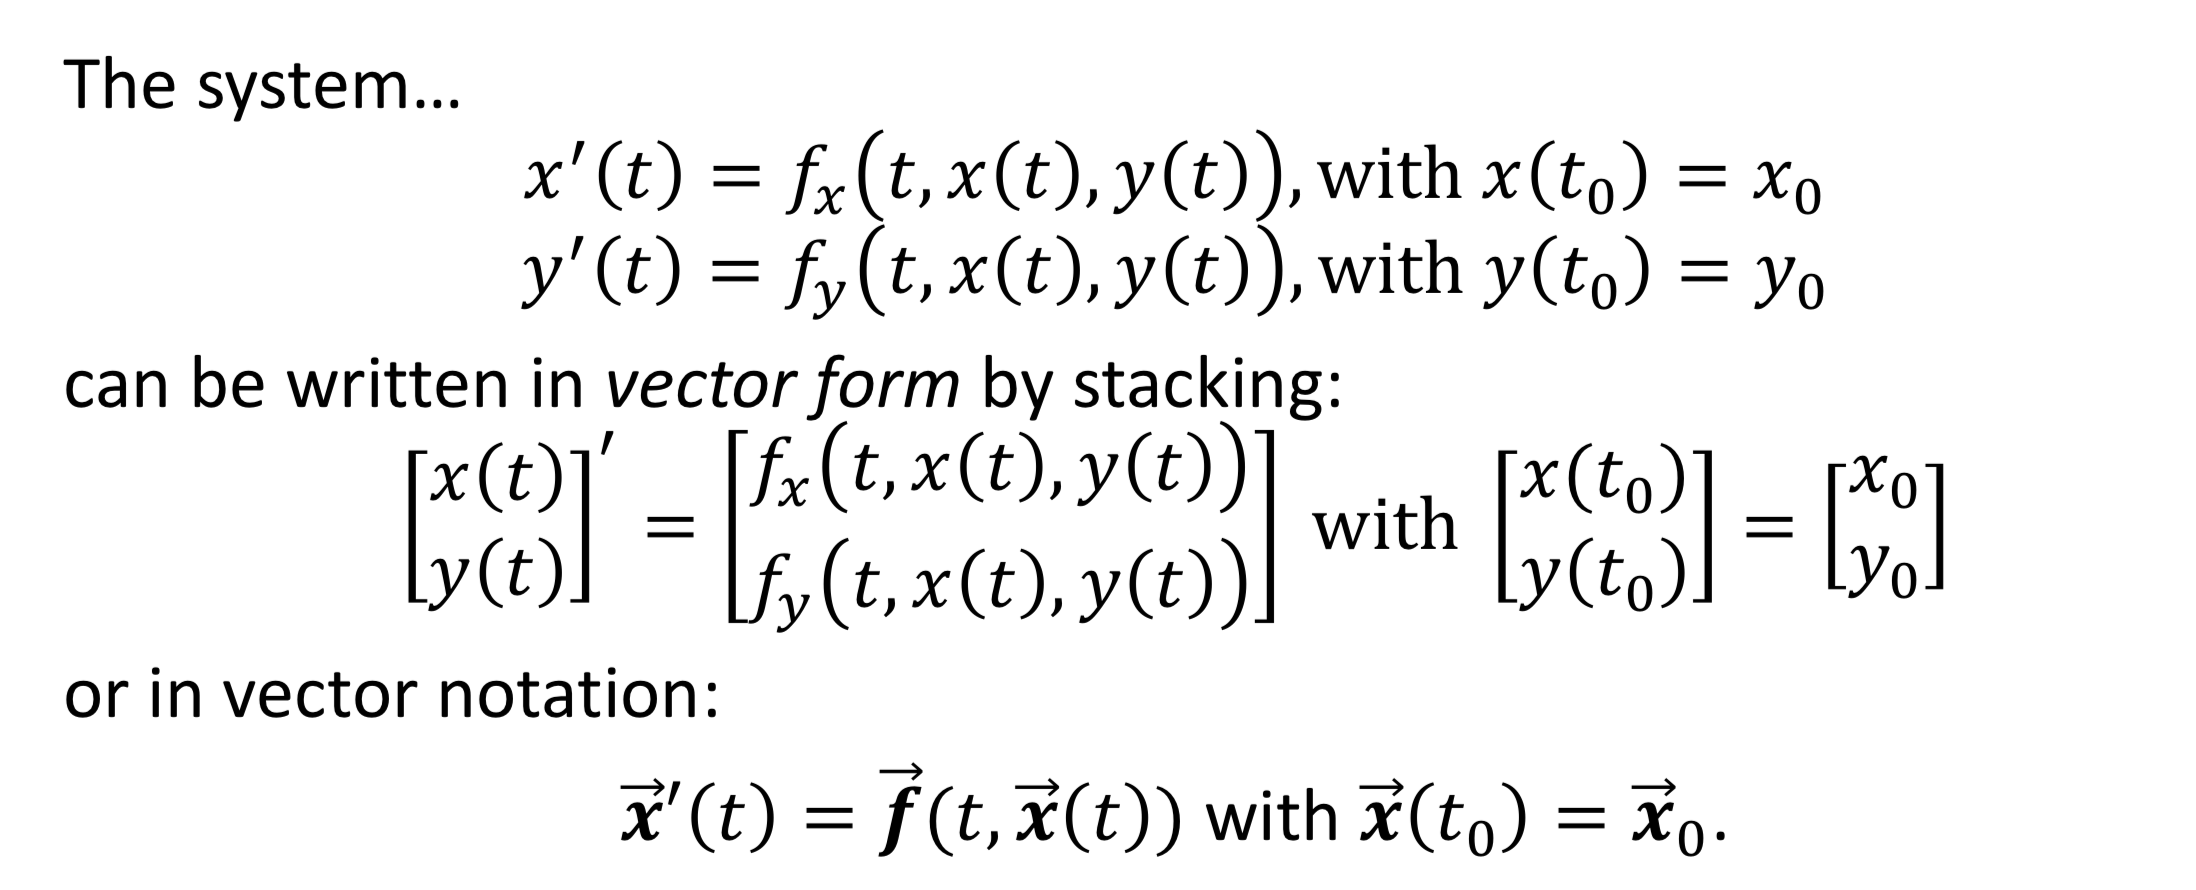
\includegraphics[scale=0.3]{1}
\end{center}

\subsubsection{Time-Stepping}
Given initial conditions, we repeatedly step sequentially forward to the next time instant, using the derivative info, \(y^\prime\) and a timestep, \(h\)

Set \(n = 0, t=t_0, y = y_0\)
\begin{enumerate}
\item Compute \(y_{n+1}\)
\item Increment time, \(t_{n+1} = t_n + h\)
\item Advance, \(n = n + 1\)
\item Repeat
\end{enumerate}

\begin{itemize}
\item Single Step Time Stepping involves using information from current time 
\item Multi Step Time Stepping involves using information from previous time steps
\item Explicit time stepping is when \(y_{n+1}\) is given as an explicit function to evaluate
\item Implicit time stepping is when \(y_{n+1}\) is not given as an explicit function to evaluate
\item Timestep Size \(h\) can be constant or Variable
\end{itemize}

\end{document}




